\section{Model Inadequacies and Transformations}


\begin{frame}{Correcting Model Inadequacies}
\begin{itemize}
    \item Least-squares inference assumes a linear relationship, constant error variance, and normally distributed errors
    \item Residual plots reveal when these assumptions fail
    \item One standard remedy is to transform the data; weighting is a separate topic
    \item In this lecture: transforming $y$ to stabilize the variance, transforming $y$ or $x$ to linearize the model, and two analytical methods for choosing the power (Box--Cox for $y$, Box--Tidwell for $x$)
\end{itemize}
\end{frame}


\begin{frame}{Recognizing Nonconstant Variance}
\begin{itemize}
    \item Plot R-student against the fitted values $\hat{y}_i$
    \item Outward-opening funnel: the spread grows with $E(y_i)$, common when $y$ is a count or an amount
    \item Double bow: the spread is largest in the middle and small at the extremes, typical when $y$ is a proportion
    \item With nonconstant variance the OLS estimators remain unbiased but are no longer minimum-variance, and the usual $t$ and $F$ tests are unreliable
\end{itemize}
\end{frame}


\begin{frame}{Idea of a Variance-Stabilizing Transformation}
\begin{itemize}
    \item Suppose $\Var(y_i)$ depends on the mean $E(y_i)$
    \item Replace $y$ by $y^* = h(y)$, with $h$ chosen so that $\Var(y^*)$ is approximately constant
    \item Then fit the model on the transformed scale
\end{itemize}
\begin{align*}
    y_i^* = \beta_0 + \beta_1 x_i + \epsilon_i, \qquad \Var(\epsilon_i) \approx \sigma^2
\end{align*}
\begin{itemize}
    \item The appropriate $h$ depends on how $\Var(y)$ is related to $E(y)$
\end{itemize}
\end{frame}



\section{Variance-Stabilizing Transformations}


\begin{frame}{Variance-Stabilizing Transformations}
\begin{center}
{\renewcommand{\arraystretch}{1.4}
\small
\begin{tabular}{ll}
\toprule
Relationship of $\sigma^2$ to $E(y)$ & Transformation \\
\midrule
$\sigma^2 \propto \text{constant}$ & $y^* = y$ (no transformation) \\
$\sigma^2 \propto E(y)$ & $y^* = \sqrt{y}$ (Poisson data) \\
$\sigma^2 \propto E(y)\,[1 - E(y)]$ & $y^* = \sin^{-1}\!\big(\sqrt{y}\,\big)$ (binomial proportions, $0 \le y_i \le 1$) \\
$\sigma^2 \propto [E(y)]^2$ & $y^* = \ln y$ \\
$\sigma^2 \propto [E(y)]^3$ & $y^* = y^{-1/2}$ \\
$\sigma^2 \propto [E(y)]^4$ & $y^* = y^{-1}$ \\
\bottomrule
\end{tabular}}
\end{center}
\end{frame}


\begin{frame}{Reading the Table}
\begin{itemize}
    \item The stronger the dependence of $\sigma^2$ on $E(y)$, the stronger the transformation: $\sqrt{y}$, then $\ln y$, then $y^{-1/2}$, then $y^{-1}$
    \item Poisson counts have $\Var(y) = E(y)$, so $\sigma^2 \propto E(y)$ and the square root applies
    \item A proportion $y = X/m$ with $X \sim \text{Binomial}(m, p)$ has $\Var(y) = p(1-p)/m$, so $\sigma^2 \propto E(y)[1 - E(y)]$ and the arcsine square root applies
    \item $\sigma^2 \propto [E(y)]^2$ means the standard deviation is proportional to the mean, which calls for the logarithm
\end{itemize}
\end{frame}


\begin{frame}{Choosing a Transformation in Practice}
\begin{enumerate}
    \item Fit the model by OLS on the original $y$ and plot R-student against $\hat{y}_i$
    \item If the pattern of spread matches a row of the table, apply that transformation
    \item Refit with $y^*$ and examine the residual plots again
    \item If the variance is still not constant, try a stronger or weaker transformation
\end{enumerate}
The exact relationship between $\sigma^2$ and $E(y)$ is rarely known, so the choice is often made by trial and error.
\end{frame}


\begin{frame}{Consequences of Transforming the Response}
\begin{itemize}
    \item Estimates and tests refer to the $y^*$ scale; for example, coefficients describe the change in $\sqrt{y}$, not in $y$
    \item To predict on the original scale, apply the inverse transformation to fitted values and to interval endpoints
    \item $R^2$ values from models with different responses cannot be compared
    \item Transforming $y$ also changes the shape of the relationship and the error distribution, so all residual checks must be repeated
\end{itemize}
\end{frame}



\section{Example: Electric Utility Data}


\begin{frame}{Electric Utility Data}
\begin{columns}[T]
\begin{column}{0.5\textwidth}
\begin{itemize}
    \item $y$: peak demand (kW), $x$: monthly energy usage (kWh)
    \item $n = 53$ residential customers in August (MPV Table 5.2)
    \item Goal: model demand as a function of usage
    \item The spread of $y$ increases with $x$
\end{itemize}
\end{column}
\begin{column}{0.5\textwidth}
\mode<presentation>{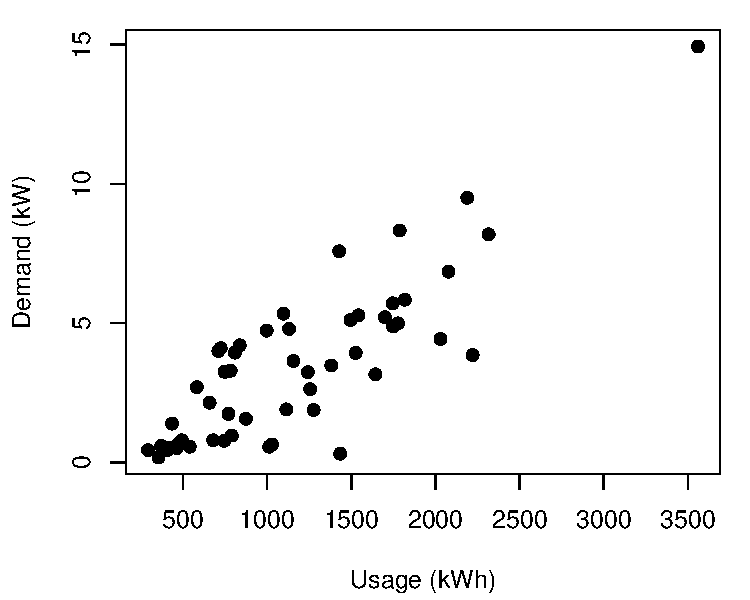
\includegraphics[width=\linewidth]{figures/eu_scatter.pdf}}
\mode<article>{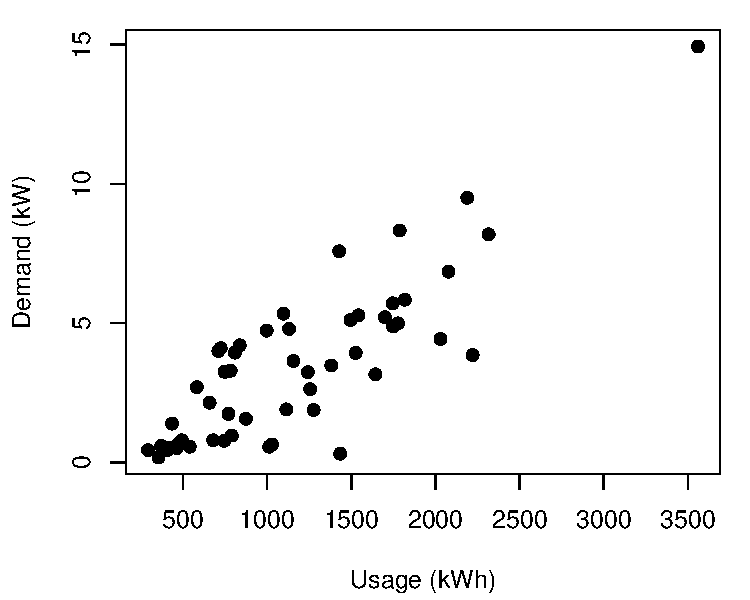
\includegraphics[width=0.8\linewidth]{figures/eu_scatter.pdf}}
\end{column}
\end{columns}
\end{frame}


\begin{frame}{Straight-Line Fit}
\begin{columns}[T]
\begin{column}{0.5\textwidth}
\begin{align*}
    \hat{y} &= -0.8313 + 0.003683\,x \\
    R^2 &= 0.7046
\end{align*}
\begin{itemize}
    \item R-student against $\hat{y}$ shows an outward-opening funnel
    \item The constant-variance assumption is violated
\end{itemize}
\end{column}
\begin{column}{0.5\textwidth}
\mode<presentation>{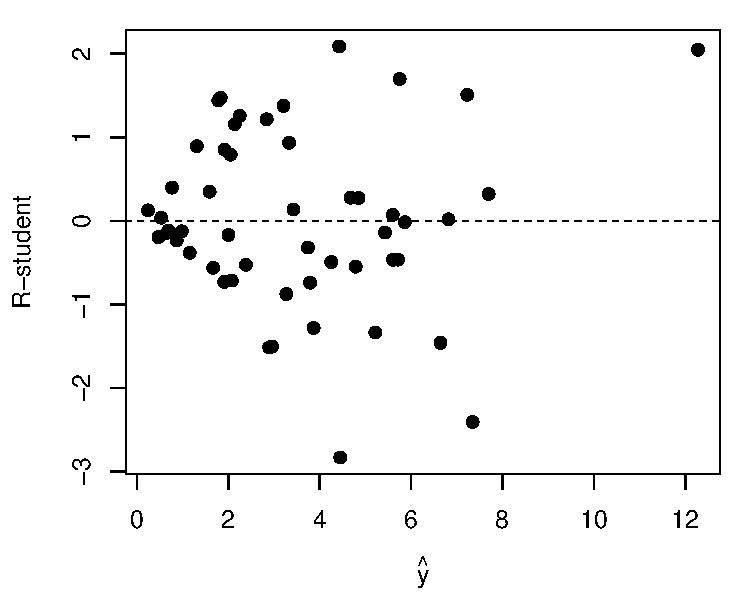
\includegraphics[width=\linewidth]{figures/eu_rstudent_original.pdf}}
\mode<article>{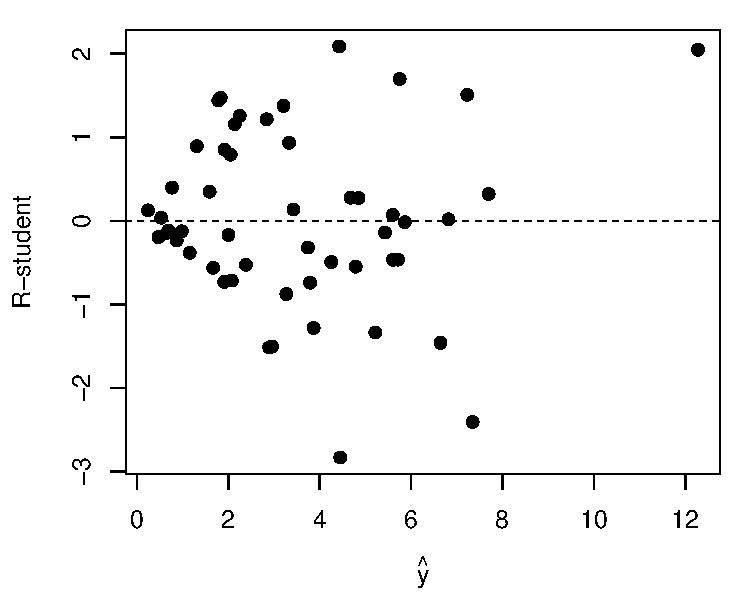
\includegraphics[width=0.8\linewidth]{figures/eu_rstudent_original.pdf}}
\end{column}
\end{columns}
\end{frame}


\begin{frame}{Question: Which Transformation?}
The residual plot is an outward-opening funnel, so the variance increases with the mean. Which row of the variance-stabilizing table would you try first, and what would you do if the funnel persisted?
% Answer:
% \begin{itemize}
%     \item Try $\sigma^2 \propto E(y)$ first, that is $y^* = \sqrt{y}$
%     \item If the funnel persists, move to the stronger transformation $\ln y$
% \end{itemize}
\end{frame}


\begin{frame}{Square-Root Transformation}
\begin{columns}[T]
\begin{column}{0.5\textwidth}
\begin{align*}
    y^* &= \sqrt{y} \\
    \hat{y}^* &= 0.5822 + 0.0009529\,x \\
    R^2 &= 0.6485
\end{align*}
\begin{itemize}
    \item R-student against $\hat{y}^*$ no longer shows a funnel
    \item The variance now looks stable
\end{itemize}
\end{column}
\begin{column}{0.5\textwidth}
\mode<presentation>{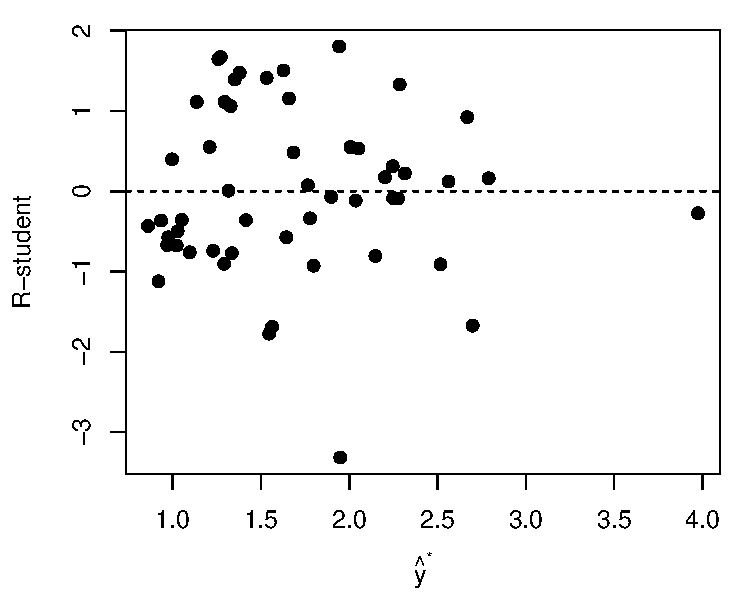
\includegraphics[width=\linewidth]{figures/eu_rstudent_sqrt.pdf}}
\mode<article>{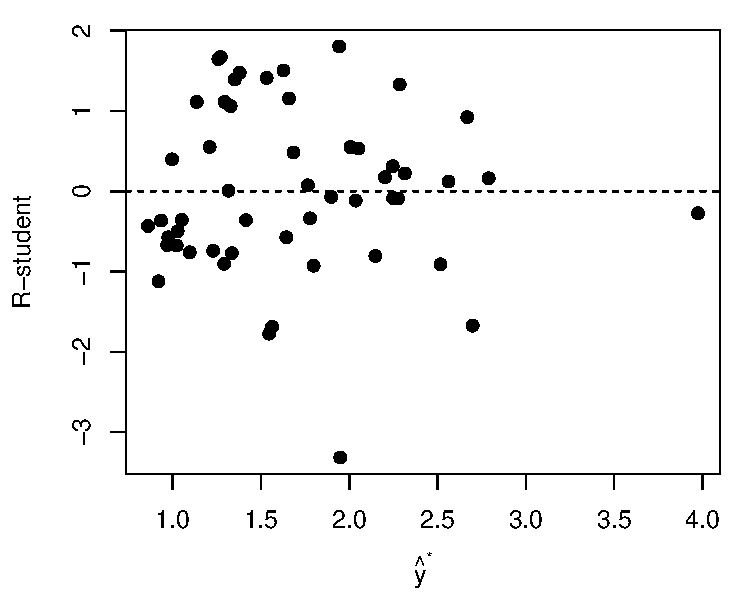
\includegraphics[width=0.8\linewidth]{figures/eu_rstudent_sqrt.pdf}}
\end{column}
\end{columns}
\end{frame}


\begin{frame}{A Stronger Transformation: $\ln y$}
\begin{columns}[T]
\begin{column}{0.5\textwidth}
\begin{align*}
    y^* &= \ln y \\
    \hat{y}^* &= -0.5587 + 0.001172\,x \\
    R^2 &= 0.5266
\end{align*}
\begin{itemize}
    \item The residual plot now shows curvature
    \item The logarithm is too strong for these data
\end{itemize}
\end{column}
\begin{column}{0.5\textwidth}
\mode<presentation>{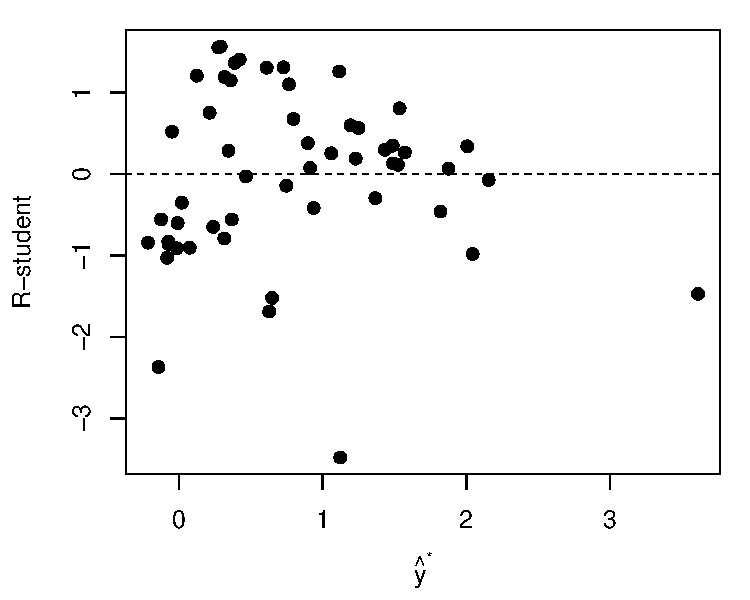
\includegraphics[width=\linewidth]{figures/eu_rstudent_log.pdf}}
\mode<article>{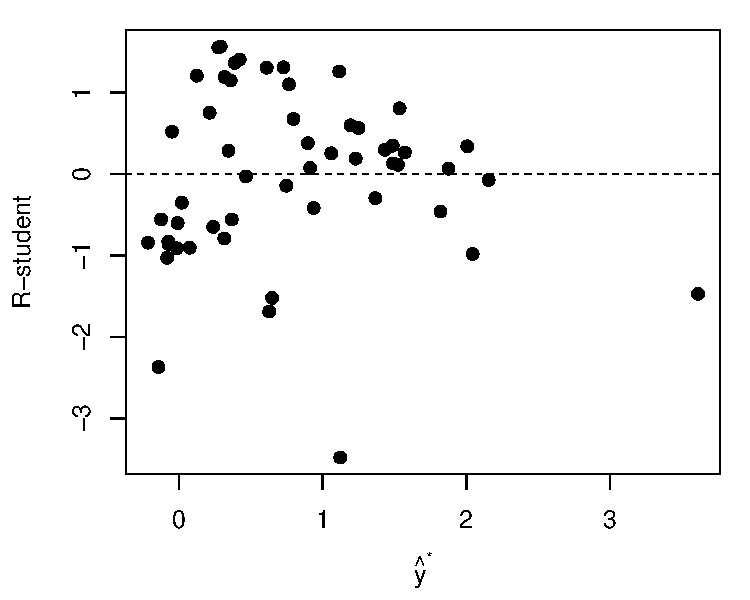
\includegraphics[width=0.8\linewidth]{figures/eu_rstudent_log.pdf}}
\end{column}
\end{columns}
\end{frame}


\begin{frame}{Question: Did $R^2$ Get Worse?}
$R^2$ dropped from $0.7046$ for $y$ to $0.6485$ for $\sqrt{y}$. Does this mean the transformed model is worse?
% Answer:
% \begin{itemize}
%     \item No: the two $R^2$ values describe different responses ($y$ and $\sqrt{y}$) and cannot be compared
%     \item The transformed model is judged by its residual diagnostics, which now satisfy the constant-variance assumption
% \end{itemize}
\end{frame}



% \section{Arcsine Transformation: Simulated Proportions}


% \begin{frame}{Simulating Proportions}
% \begin{itemize}
%     \item $y_i = X_i/m$ with $X_i \sim \text{Binomial}(m, p_i)$ and $m = 20$
%     \item $p_i = 0.05 + 0.90\,x_i$, with $x_i$ at 10 equally spaced points in $[0, 1]$ and 30 replicates at each ($n = 300$)
% \end{itemize}
% \begin{align*}
%     E(y_i) = p_i, \qquad \Var(y_i) = \frac{p_i(1 - p_i)}{m}
% \end{align*}
% \begin{itemize}
%     \item So $\sigma^2 \propto E(y)[1 - E(y)]$, and the table suggests $y^* = \sin^{-1}\!\big(\sqrt{y}\,\big)$
% \end{itemize}
% \end{frame}


% \begin{frame}{Variance Before and After the Transformation}
% \begin{columns}[T]
% \begin{column}{0.5\textwidth}
% \centering
% Original $y$

% \mode<presentation>{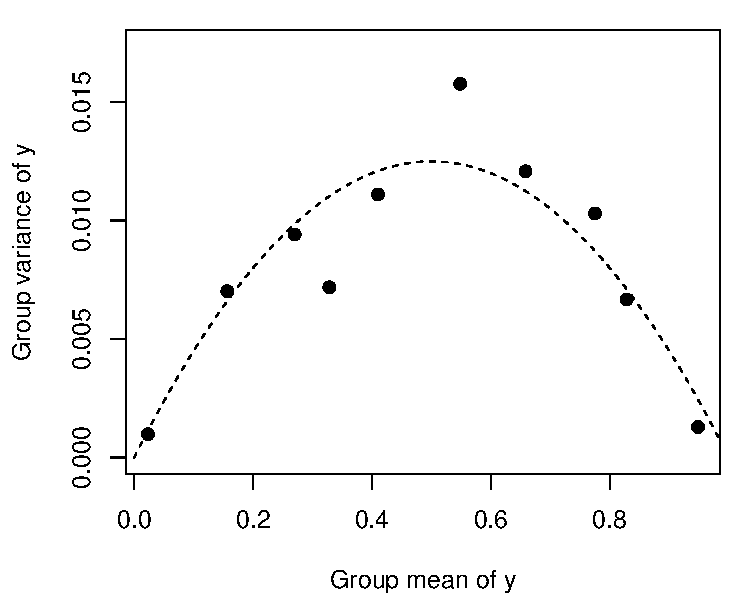
\includegraphics[width=0.8\linewidth]{figures/as_variance_original.pdf}}
% \mode<article>{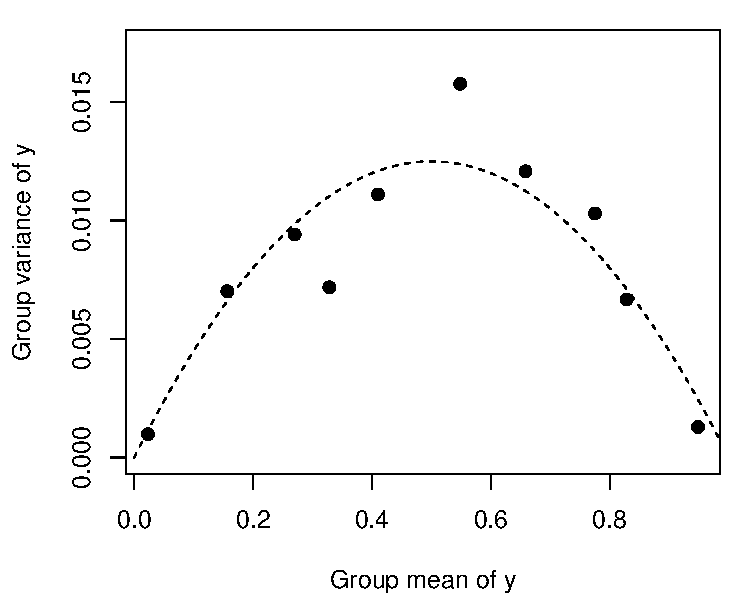
\includegraphics[width=0.9\linewidth]{figures/as_variance_original.pdf}}
% \end{column}
% \begin{column}{0.5\textwidth}
% \centering
% $y^* = \sin^{-1}\!\big(\sqrt{y}\,\big)$

% \mode<presentation>{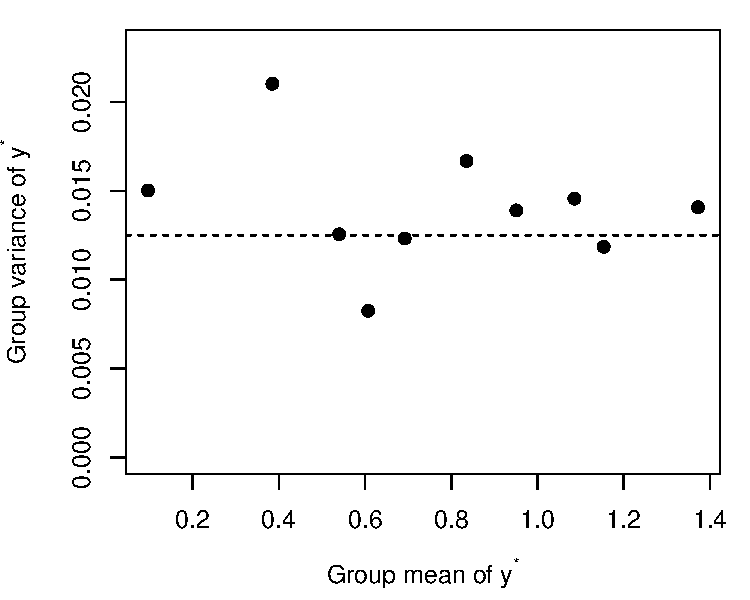
\includegraphics[width=0.8\linewidth]{figures/as_variance_transformed.pdf}}
% \mode<article>{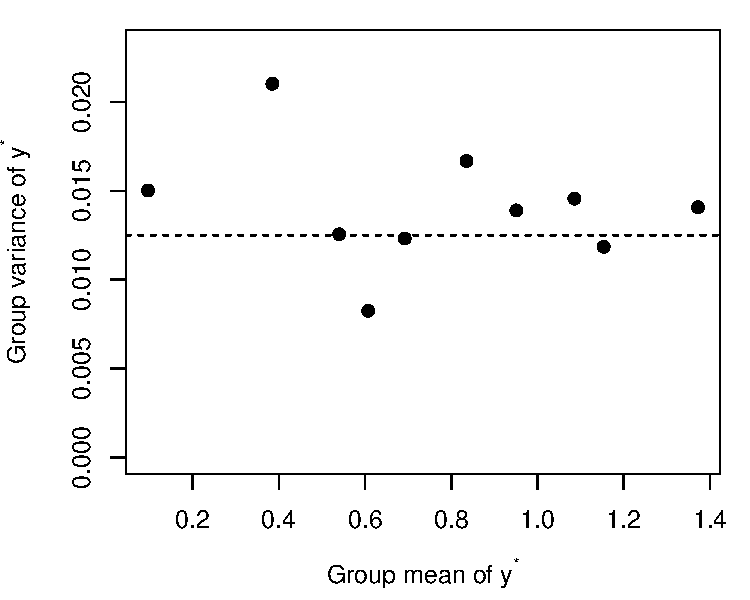
\includegraphics[width=0.9\linewidth]{figures/as_variance_transformed.pdf}}
% \end{column}
% \end{columns}
% \begin{itemize}
%     \item Each point: sample variance at one design point against the group mean
%     \item Left: the variance rises and then falls (dashed: $p(1-p)/m$)
%     \item Right: the variance is roughly constant (dashed: approximately $1/(4m)$)
% \end{itemize}
% \end{frame}


% \begin{frame}{Residuals Before and After the Transformation}
% \begin{columns}[T]
% \begin{column}{0.5\textwidth}
% \centering
% Original $y$

% \mode<presentation>{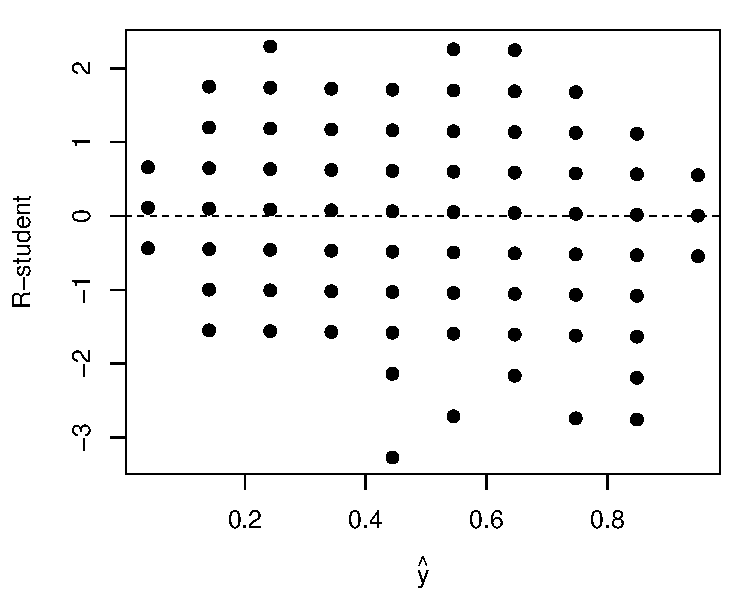
\includegraphics[width=\linewidth]{figures/as_rstudent_original.pdf}}
% \mode<article>{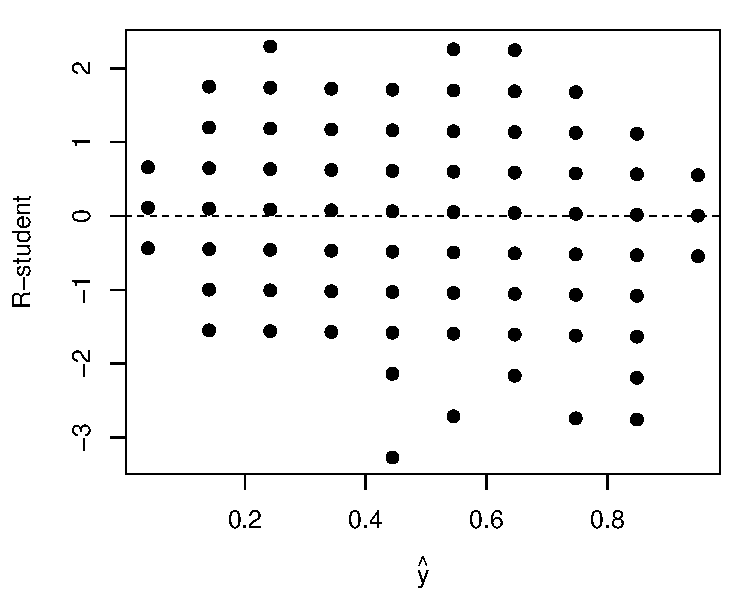
\includegraphics[width=0.9\linewidth]{figures/as_rstudent_original.pdf}}
% \end{column}
% \begin{column}{0.5\textwidth}
% \centering
% $y^* = \sin^{-1}\!\big(\sqrt{y}\,\big)$

% \mode<presentation>{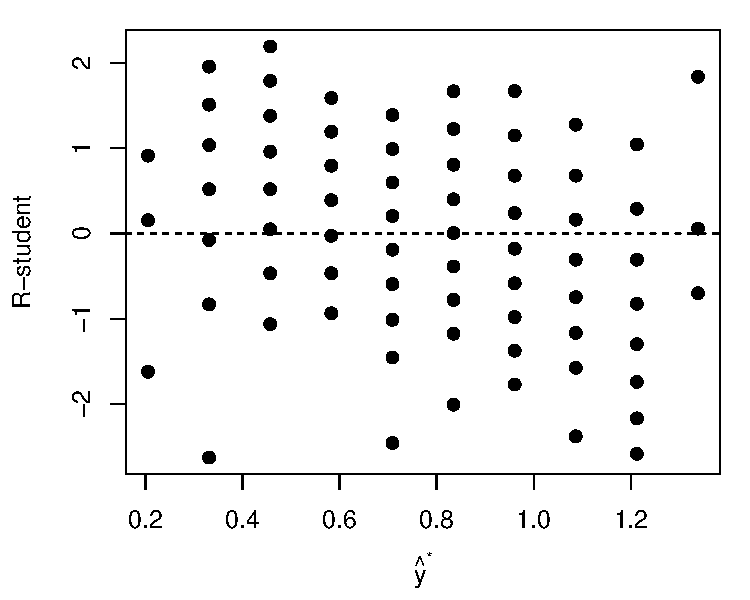
\includegraphics[width=\linewidth]{figures/as_rstudent_transformed.pdf}}
% \mode<article>{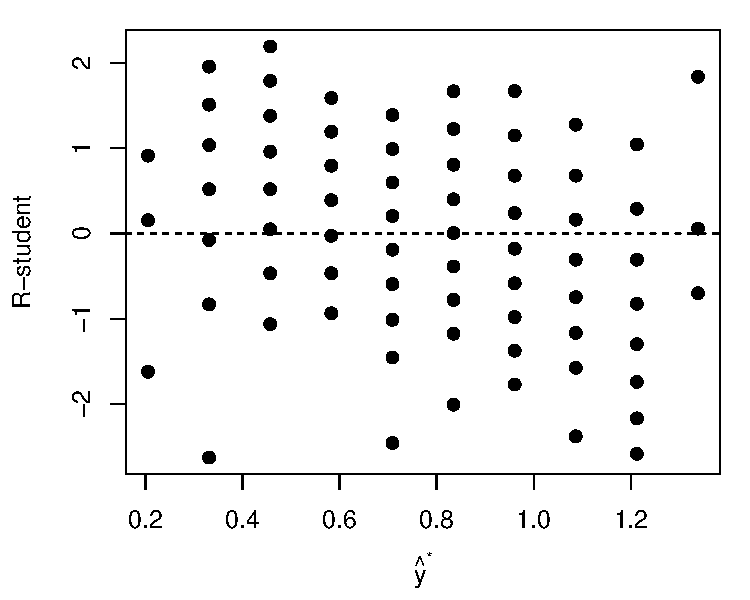
\includegraphics[width=0.9\linewidth]{figures/as_rstudent_transformed.pdf}}
% \end{column}
% \end{columns}
% \begin{itemize}
%     \item Original: the spread narrows at the extremes of $\hat{y}$ (double bow)
%     \item Transformed: the spread is more even across the fitted values
% \end{itemize}
% \end{frame}



\section{Transformations to Linearize the Model}


\begin{frame}{Linearizable Nonlinear Functions}
\begin{center}
{\renewcommand{\arraystretch}{1.4}
\small
\begin{tabular}{lll}
\toprule
Function & Transformation & Linear form \\
\midrule
$y = \beta_0 x^{\beta_1}$ & $y' = \log y$, $x' = \log x$ & $y' = \log \beta_0 + \beta_1 x'$ \\
$y = \beta_0 e^{\beta_1 x}$ & $y' = \ln y$ & $y' = \ln \beta_0 + \beta_1 x$ \\
$y = \beta_0 + \beta_1 \log x$ & $x' = \log x$ & $y = \beta_0 + \beta_1 x'$ \\
$y = \dfrac{x}{\beta_0 x - \beta_1}$ & $y' = \dfrac{1}{y}$, $x' = \dfrac{1}{x}$ & $y' = \beta_0 - \beta_1 x'$ \\
\bottomrule
\end{tabular}}
\end{center}
\end{frame}


\begin{frame}{The Error Structure Matters}
\begin{itemize}
    \item Linearizing the exponential function assumes the error is multiplicative
\end{itemize}
\begin{align*}
    y = \beta_0 e^{\beta_1 x}\,\epsilon \quad\Longrightarrow\quad \ln y = \ln \beta_0 + \beta_1 x + \ln \epsilon
\end{align*}
\begin{itemize}
    \item The linearized model is appropriate if $\ln \epsilon$ has mean zero, constant variance, and is normal
    \item If instead the error is additive, $y = \beta_0 e^{\beta_1 x} + \epsilon$, taking logarithms does not give a linear model with additive error, and nonlinear regression is needed
\end{itemize}
\end{frame}


\begin{frame}{Transform $x$ or Transform $y$?}
\begin{itemize}
    \item Transforming $x$ alone leaves the distribution of the errors unchanged
    \item Transforming $y$ changes both the shape of the relationship and the error distribution
    \item Curved scatter with roughly constant variance: transform $x$
    \item Curved scatter with nonconstant variance: transform $y$, which may fix both problems
\end{itemize}
\end{frame}



\section{Example: Windmill Data}


\begin{frame}{Windmill Data}
\begin{columns}[T]
\begin{column}{0.5\textwidth}
\begin{itemize}
    \item $y$: DC output of a windmill, $x$: wind velocity (mph)
    \item $n = 25$ observations (MPV Table 5.5)
    \item Goal: model DC output as a function of wind velocity
    \item The scatter plot is clearly curved
\end{itemize}
\end{column}
\begin{column}{0.5\textwidth}
\mode<presentation>{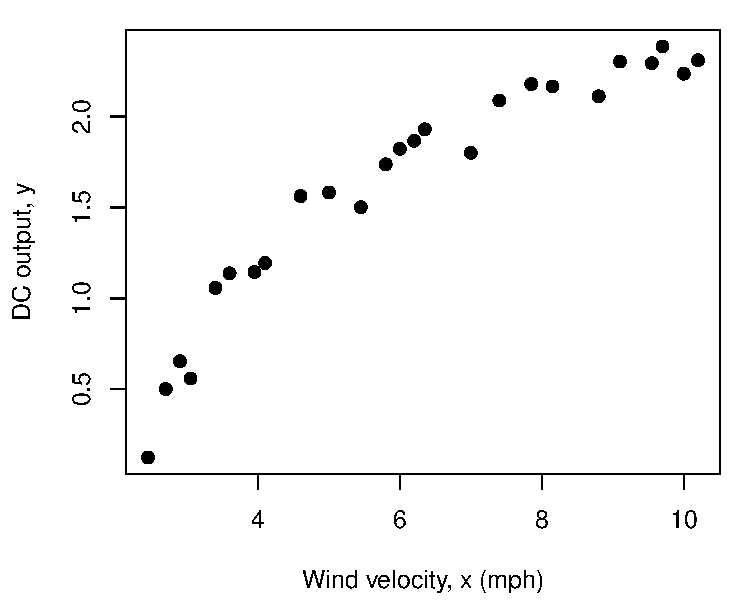
\includegraphics[width=\linewidth]{figures/wm_scatter.pdf}}
\mode<article>{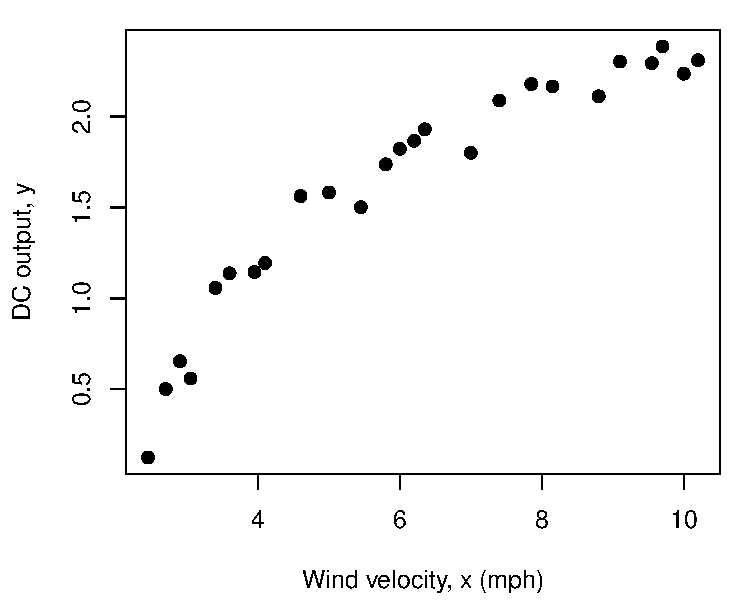
\includegraphics[width=0.8\linewidth]{figures/wm_scatter.pdf}}
\end{column}
\end{columns}
\end{frame}


\begin{frame}{Question: Which Transformation?}
DC output rises with wind velocity but levels off, and the spread around the trend looks roughly constant. Which transformation would you try, and on which variable?
% Answer:
% \begin{itemize}
%     \item The curve approaches an upper limit, which matches the form $y = x/(\beta_0 x - \beta_1)$
%     \item The spread looks constant, so transform $x$ only: $x' = 1/x$
% \end{itemize}
\end{frame}


\begin{frame}{Straight-Line Fit}
\begin{columns}[T]
\begin{column}{0.5\textwidth}
\begin{align*}
    \hat{y} &= 0.1309 + 0.2411\,x \\
    R^2 &= 0.8745
\end{align*}
\begin{itemize}
    \item R-student against $\hat{y}$ shows a clear curved pattern
    \item The straight line is inadequate despite the high $R^2$
\end{itemize}
\end{column}
\begin{column}{0.5\textwidth}
\mode<presentation>{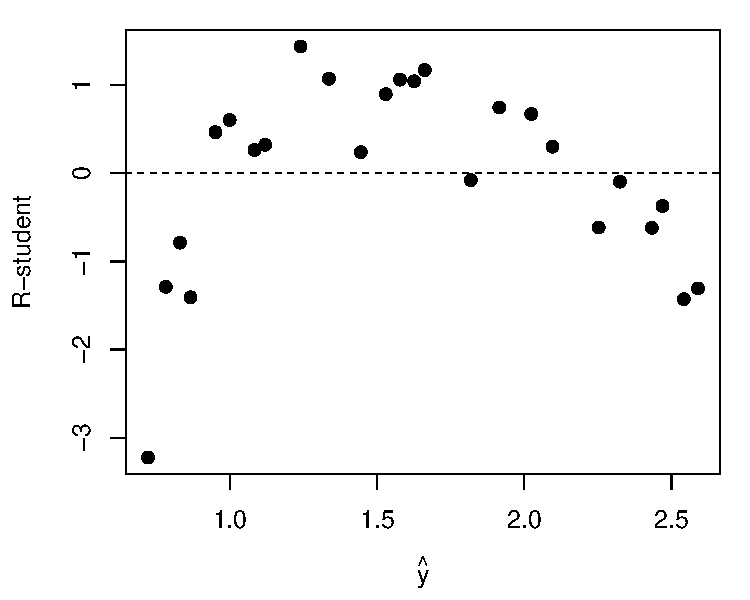
\includegraphics[width=\linewidth]{figures/wm_rstudent_linear.pdf}}
\mode<article>{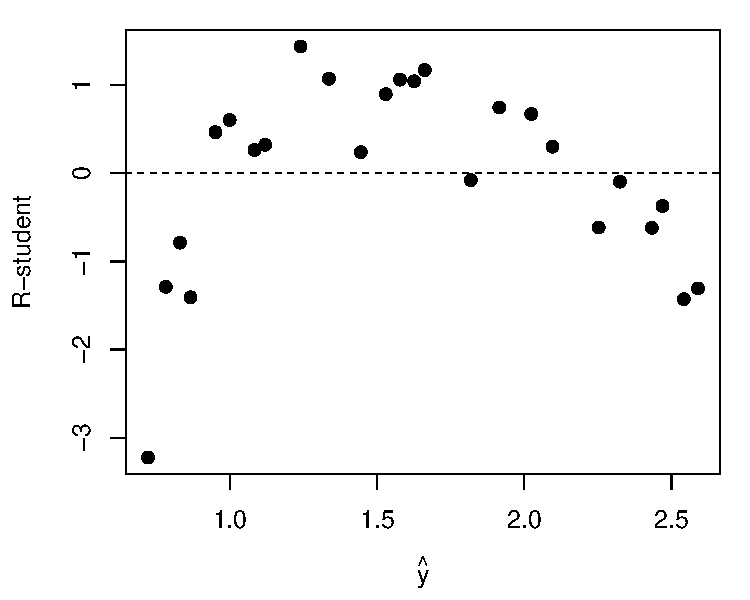
\includegraphics[width=0.8\linewidth]{figures/wm_rstudent_linear.pdf}}
\end{column}
\end{columns}
\end{frame}


\begin{frame}{Reciprocal Transformation of $x$}
\begin{columns}[T]
\begin{column}{0.5\textwidth}
\begin{align*}
    x' &= 1/x \\
    \hat{y} &= 2.9789 - 6.9345\,x' \\
    R^2 &= 0.9800
\end{align*}
\begin{itemize}
    \item The scatter plot against $x'$ is close to a straight line
    \item As $x \to \infty$ the fitted output approaches $2.9789$, the upper limit
\end{itemize}
\end{column}
\begin{column}{0.5\textwidth}
\mode<presentation>{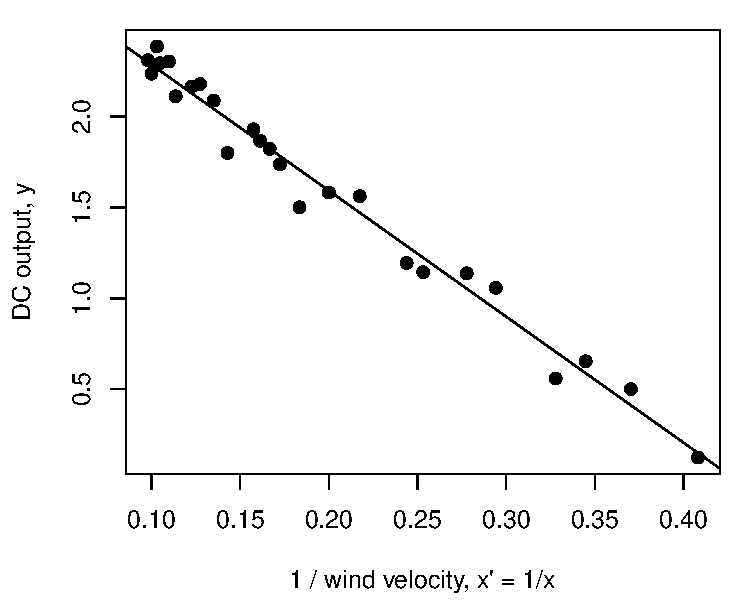
\includegraphics[width=\linewidth]{figures/wm_scatter_inverse.pdf}}
\mode<article>{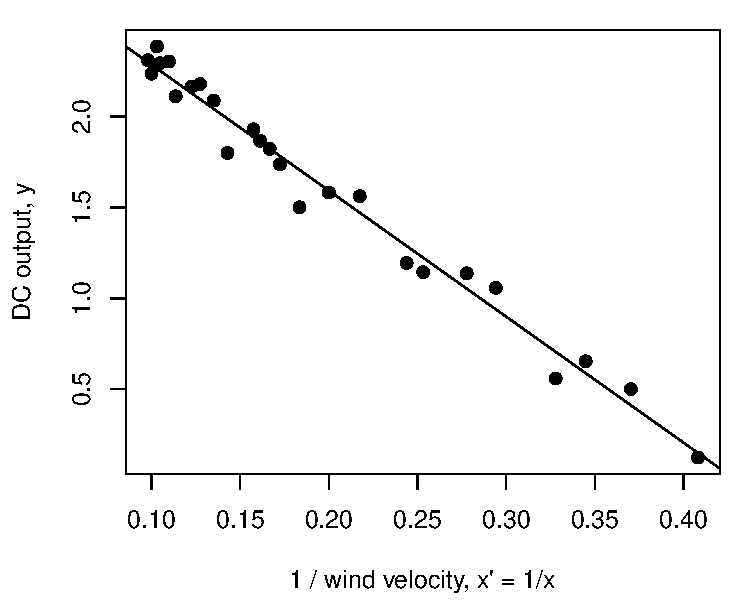
\includegraphics[width=0.8\linewidth]{figures/wm_scatter_inverse.pdf}}
\end{column}
\end{columns}
\end{frame}


\begin{frame}{Residual Analysis After the Transformation}
\begin{columns}[T]
\begin{column}{0.5\textwidth}
\mode<presentation>{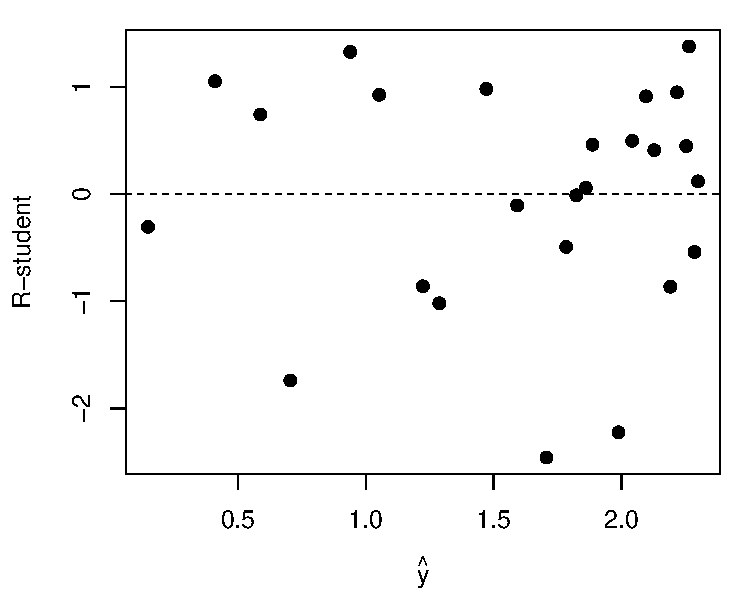
\includegraphics[width=\linewidth]{figures/wm_rstudent_inverse.pdf}}
\mode<article>{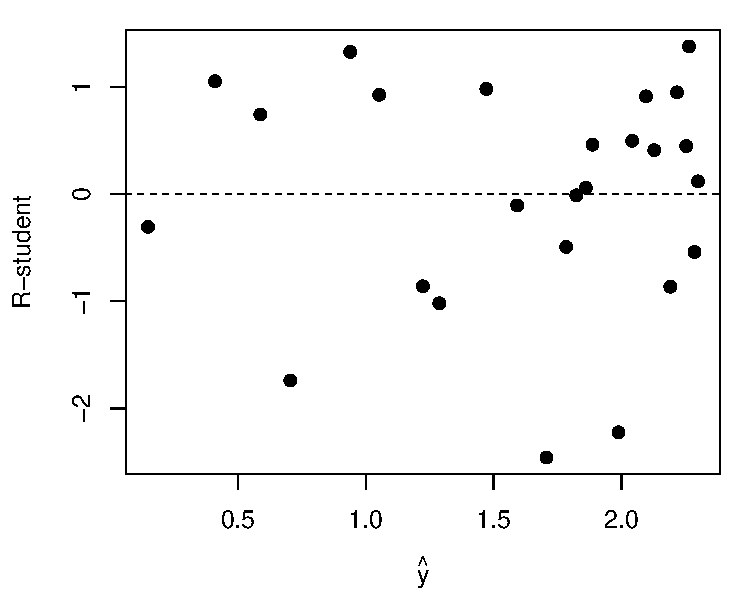
\includegraphics[width=0.9\linewidth]{figures/wm_rstudent_inverse.pdf}}
\end{column}
\begin{column}{0.5\textwidth}
\mode<presentation>{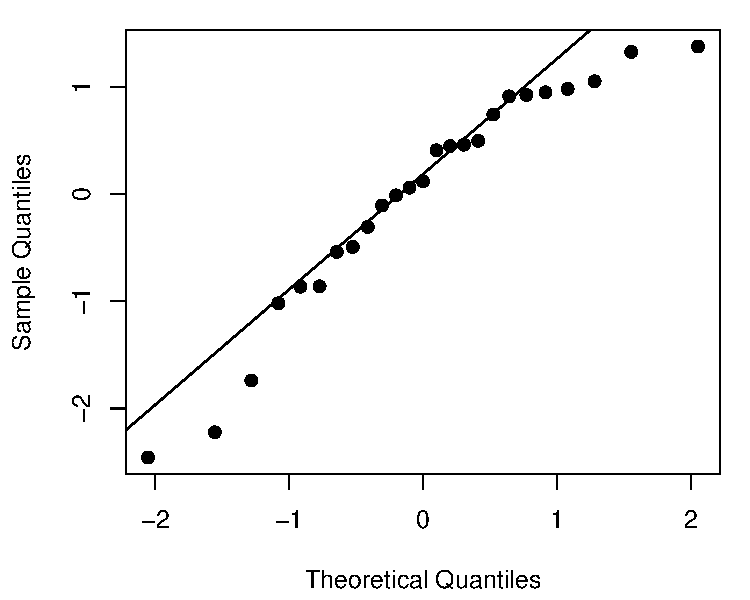
\includegraphics[width=\linewidth]{figures/wm_qq_inverse.pdf}}
\mode<article>{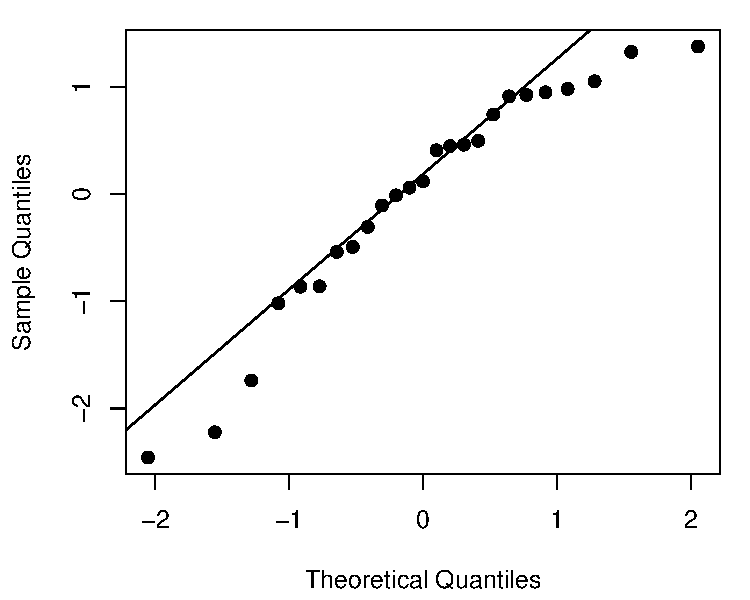
\includegraphics[width=0.9\linewidth]{figures/wm_qq_inverse.pdf}}
\end{column}
\end{columns}
\begin{itemize}
    \item R-student against $\hat{y}$ shows no systematic pattern
    \item The normal probability plot is close to a straight line
\end{itemize}
\end{frame}



\section{The Box--Cox Method}


\begin{frame}{Motivation for the Box--Cox Method}
\begin{itemize}
    \item The variance-stabilizing table requires knowing how $\sigma^2$ depends on $E(y)$, which is usually unknown
    \item Box and Cox (1964): estimate the power of the transformation from the data
    \item Considers the power family $y^\lambda$, with $\lambda$ estimated together with $\bbeta$ by maximum likelihood
    \item Aims to correct nonnormality and nonconstant variance, and requires $y_i > 0$
\end{itemize}
\end{frame}


\begin{frame}{The Power Transformation Family}
\begin{align*}
    y^{(\lambda)} =
    \begin{cases}
        \dfrac{y^\lambda - 1}{\lambda}, & \lambda \neq 0 \\[1ex]
        \ln y, & \lambda = 0
    \end{cases}
\end{align*}
\begin{itemize}
    \item As $\lambda \to 0$, $(y^\lambda - 1)/\lambda \to \ln y$, so the logarithm belongs to the family
    \item $\lambda = 1$: no transformation, $\lambda = 1/2$: square root, $\lambda = -1$: reciprocal
\end{itemize}
\end{frame}


\begin{frame}{The Scaled Response}
\begin{itemize}
    \item The size of $y^\lambda$ changes with $\lambda$, so $\SSRes$ is not comparable across values of $\lambda$
    \item Fix: divide by a factor involving the geometric mean $\dot{y}$
\end{itemize}
\begin{align*}
    y^{(\lambda)} =
    \begin{cases}
        \dfrac{y^\lambda - 1}{\lambda\,\dot{y}^{\lambda - 1}}, & \lambda \neq 0 \\[1ex]
        \dot{y} \ln y, & \lambda = 0
    \end{cases}
    \qquad
    \dot{y} = \exp\!\left[\frac{1}{n}\sum_{i=1}^{n} \ln y_i\right]
\end{align*}
\end{frame}


\begin{frame}{Model and Estimation}
\begin{align*}
    \by^{(\lambda)} = \bX\bbeta + \boldsymbol{\epsilon}, \qquad \boldsymbol{\epsilon} \sim N(\mathbf{0}, \sigma^2 \mathbf{I})
\end{align*}
\begin{itemize}
    \item For fixed $\lambda$, $\hat{\bbeta} = (\bX'\bX)^{-1}\bX'\by^{(\lambda)}$
    \item Let $\SSRes(\lambda)$ be the residual sum of squares from this fit
\end{itemize}
\begin{align*}
    \SSRes(\lambda) = \sum_{i=1}^{n} \big( y_i^{(\lambda)} - \hat{y}_i^{(\lambda)} \big)^2
\end{align*}
\begin{itemize}
    \item With the scaled response, the maximum likelihood estimate $\hat{\lambda}$ is the value that minimizes $\SSRes(\lambda)$
\end{itemize}
\end{frame}


\begin{frame}{The Box--Cox Procedure}
\begin{enumerate}
    \item Choose a grid of values of $\lambda$, for example from $-2$ to $2$
    \item For each $\lambda$, compute the scaled $y^{(\lambda)}$, fit the model, and record $\SSRes(\lambda)$
    \item Plot $\SSRes(\lambda)$ against $\lambda$ and locate the minimum $\hat{\lambda}$
    \item Analyze the simple power $y^\lambda$ (not the scaled version), using a convenient value of $\lambda$ near $\hat{\lambda}$, and recheck the residuals
\end{enumerate}
Later inference treats $\lambda$ as known, so it is only approximate.
\end{frame}


\begin{frame}{Confidence Interval for $\lambda$}
\begin{align*}
    SS^* = \SSRes(\hat{\lambda})\left(1 + \frac{t_{\alpha/2,\,\nu}^2}{\nu}\right)
\end{align*}
\begin{itemize}
    \item $\nu$ is the residual degrees of freedom
    \item A $100(1-\alpha)\%$ confidence interval for $\lambda$ contains all $\lambda$ with $\SSRes(\lambda) \le SS^*$
    \item If the interval contains $1$, no transformation is needed
    \item Otherwise choose a convenient value inside the interval, such as $-1$, $0$, $1/2$
\end{itemize}
\end{frame}


\begin{frame}{Log-Likelihood Form and \texttt{MASS::boxcox}}
\begin{itemize}
    \item Up to a constant, the profile log-likelihood of $\lambda$ is
\end{itemize}
\begin{align*}
    L(\lambda) = -\frac{n}{2} \ln \SSRes(\lambda)
\end{align*}
\begin{itemize}
    \item The likelihood-based interval keeps all $\lambda$ with $L(\hat{\lambda}) - L(\lambda) \le \tfrac{1}{2}\chi^2_{\alpha,\,1}$
    \item Equivalently, $\SSRes(\lambda) \le \SSRes(\hat{\lambda})\exp\!\big(\chi^2_{\alpha,\,1}/n\big)$, which agrees closely with $SS^*$ unless $n$ is small
    \item \texttt{MASS::boxcox} plots $L(\lambda)$ with this 95\% interval
\end{itemize}
\end{frame}



\section{Example: Box--Cox on the Electric Utility Data}


\begin{frame}{$\SSRes(\lambda)$ for the Electric Utility Data}
\begin{center}
{\renewcommand{\arraystretch}{1.2}
\small
\begin{tabular}{rr}
\toprule
$\lambda$ & $\SSRes(\lambda)$ \\
\midrule
$-1$ & $986.03$ \\
$-0.5$ & $291.58$ \\
$0$ & $134.09$ \\
$0.25$ & $107.21$ \\
$0.5$ & $96.95$ \\
$0.75$ & $101.69$ \\
$1$ & $126.87$ \\
\bottomrule
\end{tabular}}
\end{center}
\begin{itemize}
    \item The scaled $\SSRes(\lambda)$ is smallest near $\lambda = 0.5$
\end{itemize}
\end{frame}


\begin{frame}{Box--Cox Plot from \texttt{MASS}}
\begin{columns}[T]
\begin{column}{0.4\textwidth}
\begin{itemize}
    \item $\hat{\lambda} = 0.55$
    \item 95\% interval: $(0.31,\ 0.78)$
    \item Contains $\lambda = 0.5$
    \item Excludes $\lambda = 1$ and $\lambda = 0$
\end{itemize}
\end{column}
\begin{column}{0.6\textwidth}
\mode<presentation>{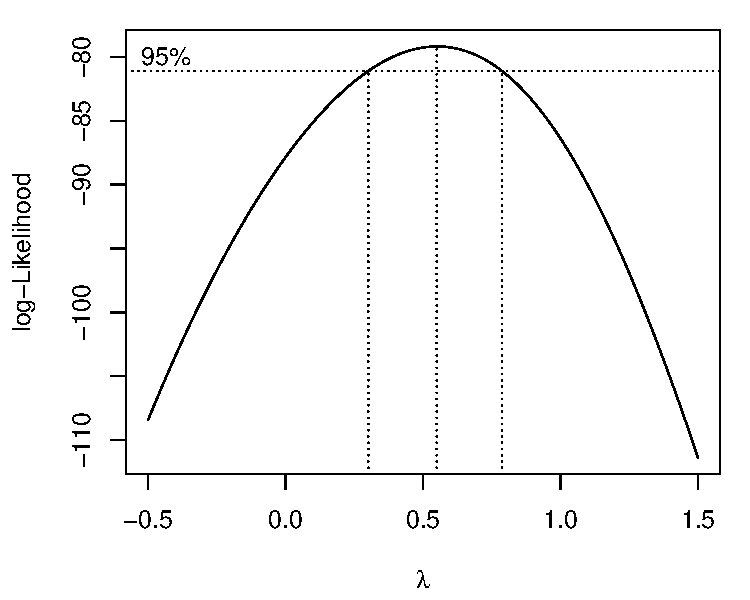
\includegraphics[width=\linewidth]{figures/eu_boxcox.pdf}}
\mode<article>{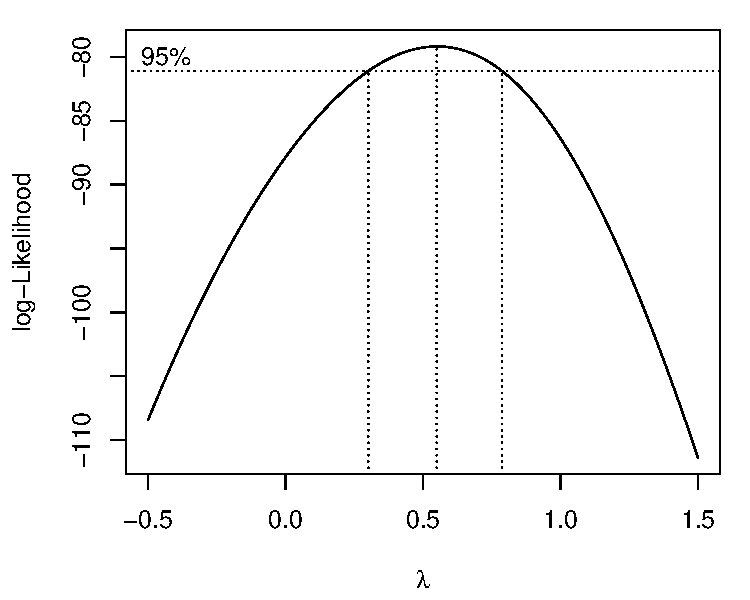
\includegraphics[width=0.8\linewidth]{figures/eu_boxcox.pdf}}
\end{column}
\end{columns}
\end{frame}


\begin{frame}{Question: Which $\lambda$ Should We Use?}
The estimate is $\hat{\lambda} = 0.55$ with 95\% interval $(0.31, 0.78)$. Which value would you use for the final model, and why?
% Answer:
% \begin{itemize}
%     \item Use $\lambda = 0.5$, that is $\sqrt{y}$: it lies inside the interval and is easy to interpret
%     \item It agrees with the transformation chosen from the residual plots and the variance-stabilizing table
%     \item The logarithm ($\lambda = 0$) and no transformation ($\lambda = 1$) are both outside the interval
% \end{itemize}
\end{frame}



\section{The Box--Tidwell Method}


\begin{frame}{Motivation for the Box--Tidwell Method}
\begin{itemize}
    \item Box--Cox transforms $y$; when the problem is nonlinearity with constant variance, transform the regressor instead
    \item Model, with unknown power $\alpha$:
\end{itemize}
\begin{align*}
    y = \beta_0 + \beta_1 \xi + \epsilon, \qquad
    \xi =
    \begin{cases}
        x^\alpha, & \alpha \neq 0 \\
        \ln x, & \alpha = 0
    \end{cases}
\end{align*}
\begin{itemize}
    \item Box and Tidwell (1962) estimate $\alpha$ iteratively
    \item Special case: $\alpha = 0$: logarithm
\end{itemize}
\end{frame}


\begin{frame}{Linearizing the Model in $\alpha$}
Expand $E(y) = \beta_0 + \beta_1 x^\alpha$ in a first-order Taylor series in $\alpha$ about $\alpha_0 = 1$, using $\partial x^\alpha / \partial \alpha = x^\alpha \ln x$:
\begin{align*}
    E(y) &\approx \beta_0 + \beta_1 x + (\alpha - 1)\,\beta_1\, x \ln x \\
    &= \beta_0 + \beta_1 x + \gamma w, \qquad \gamma = (\alpha - 1)\beta_1, \quad w = x \ln x
\end{align*}
The model is now linear in the regressors $x$ and $w$, and $\alpha = \gamma/\beta_1 + 1$.
\end{frame}


\begin{frame}{One Iteration of the Procedure}
\begin{enumerate}
    \item Fit $y = \beta_0 + \beta_1 x + \epsilon$ and record $\hat{\beta}_1$
    \item Fit $y = \beta_0^* + \beta_1^* x + \gamma w + \epsilon$ with $w = x \ln x$ and record $\hat{\gamma}$
    \item Compute the first estimate of the power
\end{enumerate}
\begin{align*}
    \hat{\alpha}_1 = \frac{\hat{\gamma}}{\hat{\beta}_1} + 1
\end{align*}
\end{frame}


\begin{frame}{Iterating}
\begin{itemize}
    \item Set $x^{(1)} = x^{\hat{\alpha}_1}$ and repeat the procedure with $x^{(1)}$ in place of $x$
    \item Stop when $\hat{\alpha}_k \approx 1$, that is, when no further transformation is needed
    \item The overall estimate is the product $\hat{\alpha} = \prod_k \hat{\alpha}_k$, since a power of a power multiplies the exponents
    \item The $t$ statistic for $\hat{\gamma}$ gives an approximate test of $H_0\colon \alpha = 1$
\end{itemize}
\end{frame}



\section{Example: Box--Tidwell on the Windmill Data}


\begin{frame}{Windmill Data: First Iteration}
\begin{align*}
    \hat{\beta}_1 = 0.2411, \qquad \hat{\gamma} = -0.4626 \quad (t = -9.13)
\end{align*}
\begin{align*}
    \hat{\alpha}_1 = \frac{-0.4626}{0.2411} + 1 = -0.918
\end{align*}
\begin{itemize}
    \item The significant $\hat{\gamma}$ confirms that the straight line is inadequate
    \item $\hat{\alpha}_1$ is close to $-1$, which suggests the reciprocal transformation
\end{itemize}
\end{frame}


\begin{frame}{Windmill Data: Iterations}
\begin{center}
{\renewcommand{\arraystretch}{1.2}
\small
\begin{tabular}{rrrrrr}
\toprule
$k$ & $\hat{\beta}_1$ & $\hat{\gamma}$ & $t(\hat{\gamma})$ & $\hat{\alpha}_k$ & cumulative $\hat{\alpha}$ \\
\midrule
1 & $0.2411$ & $-0.4626$ & $-9.13$ & $-0.9183$ & $-0.9183$ \\
2 & $-6.6784$ & $0.5994$ & $0.51$ & $0.9103$ & $-0.8359$ \\
3 & $-6.4738$ & $0.0190$ & $0.02$ & $0.9971$ & $-0.8334$ \\
4 & $-6.4686$ & $0.0006$ & $0.00$ & $0.9999$ & $-0.8333$ \\
\bottomrule
\end{tabular}}
\end{center}
\begin{itemize}
    \item From the second iteration on, $\hat{\gamma}$ is not significant and $\hat{\alpha}_k \approx 1$
    \item The procedure converges to $\hat{\alpha} = -0.833$
\end{itemize}
\end{frame}


\begin{frame}{Box--Tidwell Fit Compared with the Reciprocal Model}
\begin{columns}[T]
\begin{column}{0.5\textwidth}
\begin{align*}
    \hat{y} &= 3.2601 - 6.4684\,x^{-0.833}
\end{align*}
\begin{center}
{\renewcommand{\arraystretch}{1.2}
\small
\begin{tabular}{lrr}
\toprule
 & $\alpha = -0.833$ & $\alpha = -1$ \\
\midrule
$R^2$ & $0.9809$ & $0.9800$ \\
$\hat{\sigma}$ & $0.0920$ & $0.0942$ \\
\bottomrule
\end{tabular}}
\end{center}
\end{column}
\begin{column}{0.5\textwidth}
\mode<presentation>{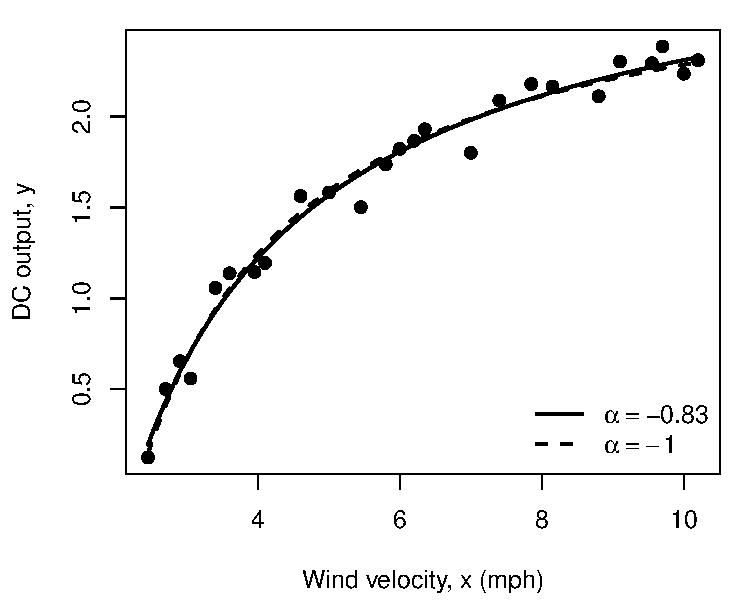
\includegraphics[width=\linewidth]{figures/wm_fit_boxtidwell.pdf}}
\mode<article>{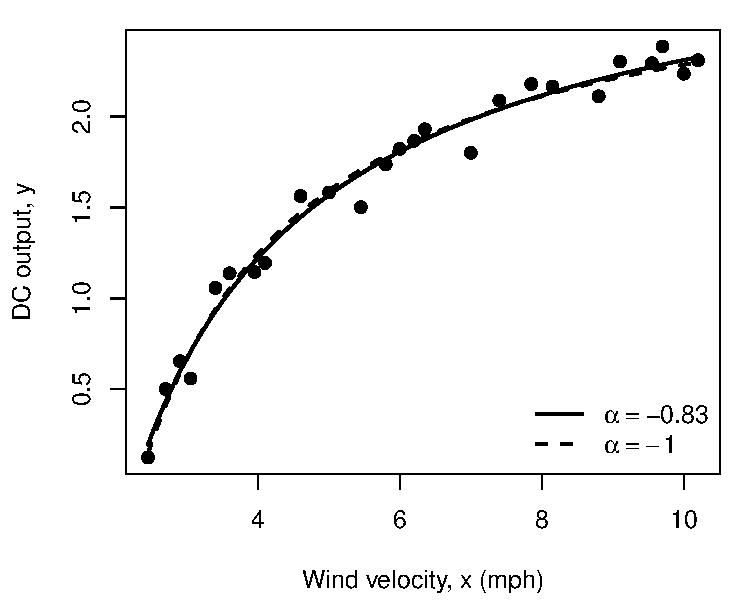
\includegraphics[width=0.8\linewidth]{figures/wm_fit_boxtidwell.pdf}}
\end{column}
\end{columns}
\end{frame}


\begin{frame}{Question: $x^{-0.833}$ or $1/x$?}
The estimated power is $-0.833$, but the reciprocal model has almost the same $R^2$. Which model would you report?
% Answer:
% \begin{itemize}
%     \item The reciprocal model: $R^2$ and $\hat{\sigma}$ are essentially unchanged and the fitted curves nearly coincide
%     \item $1/x$ is simpler to interpret and the intercept is the upper limit of DC output
% \end{itemize}
\end{frame}



\section{Summary}


\begin{frame}{Summary}
\begin{itemize}
    \item Nonconstant variance: transform $y$ using the variance-stabilizing table, then recheck the residuals
    \item Unknown variance--mean relationship: estimate the power of $y$ with the Box--Cox method
    \item Curved relationship with constant variance: transform $x$, guided by the shape of the scatter plot
    \item Unknown power for $x$: estimate it with the Box--Tidwell method
    \item After any transformation, repeat the residual analysis and interpret results on the transformed scale
\end{itemize}
\end{frame}
